\section{Preprocessing} \label{sec:chp2-sec2}
Data preprocessing is an essential and important step in machine learning. 
This step ensures the quality of the data before further analysis and serves to compensate their imperfections. 
Thus, preprocessing acts as a foundation and assures precision in the developed framework.
In our research, samples are represented by images that must be preprocessed prior to further analysis to account for artifacts and variations in the images acquisition.
Moreover, despite that some studies treated image segmentation as an individual step~\cite{barata2013towards,capdehourat2009pigmented,celebi2007methodological}, we consider it as part of the preprocessing step, alongside image enhancement, denoising, and hair removal.
%Image enhancement, hair removal and segmentation are explained in the following as part of the preprocessing step.

%However in some studies it is treated as individual step.
%Image enhancement, hair removal and segmentation are explained in the following as part of preprocessing step.


\subsection{Image enhancement}\label{subsec:pp-enh}
Image enhancement is a set of adjustment processes on an image that make it more suitable for a specific application. 
Histogram equalization, gamma transformation, contrast and edge enhancement, illumination correction, white and color balancing, color calibration, as well as denoising belong to image enhancement techniques. 
%Contrast and edge enhancement or smoothing can be applied in frequency or spatial domain. 
In the field of skin imaging, among the aforementioned techniques, median filtering is mostly used to suppress noise, bright spots, reflections and small pores on the skin ~\cite{Chiem2007,Berenguer2009,Ruiz2011}. 
While this technique removes certain noise and artifacts, it also smooths the texture and border of the lesion, which is undesirable. 
%Probably, from lesion diagnosis point of view, the most important enhancement which can be applied is color calibration and correction. 
From the lesions diagnosis point of view, perhaps the most important enhancement concerns color calibration and correction. 
This operation aims to recover real colors of an image, allowing for more reliable use of color information in manual and automatic diagnosis~\cite{korotkov2012computerized}. 
The need for color correction while using the \acf{jpeg} format as opposed to RAW images was recently highlighted in~\cite{Quintana2011,Wighton2011a,celebiautomated}.
Figure~\ref{fig:Quintana1} shows \acf{awb}, \acf{cwb} and \ac{jpeg} color calibrated dermoscopic images acquired with two polarized cameras, while 
Fig.~\ref{fig:Quintana2} demonstrates the importance of calibrating RAW data in comparison with \ac{jpeg} dermoscopic images.



\begin{figure}
\centering
\subfloat[\ac{awb}]{
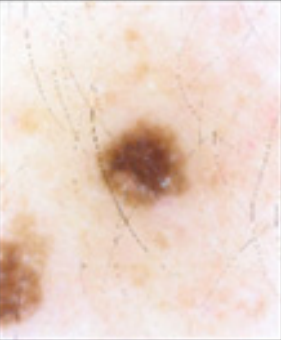
\includegraphics[height = 0.18\textheight, width= 0.16\textwidth]{Chapter2/Figures/quintana-awb_ex1.png}}\
\subfloat[\ac{cwb}]{
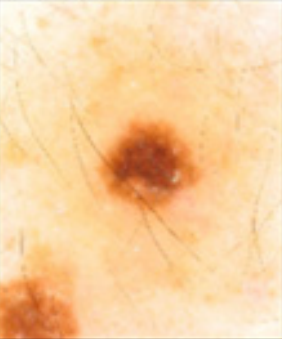
\includegraphics[height = 0.18\textheight, width= 0.16\textwidth]{Chapter2/Figures/quintana-cwb_ex1.png}}\
\subfloat[calibrated]{
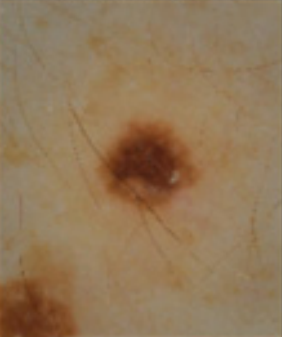
\includegraphics[height = 0.18\textheight, width= 0.16\textwidth]{Chapter2/Figures/quintana-calibrated_ex1.png}}\\
\subfloat[\ac{awb}]{
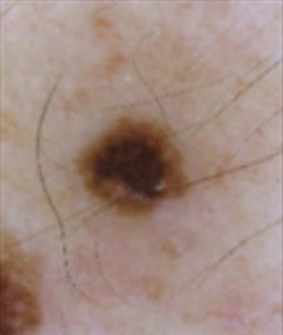
\includegraphics[height = 0.18\textheight, width= 0.16\textwidth]{Chapter2/Figures/quintana-awb_ex2.png}}\
\subfloat[\ac{cwb}]{
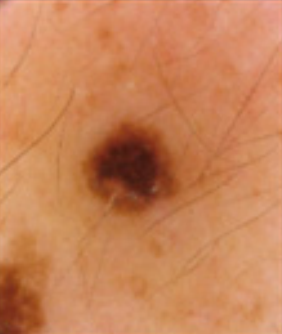
\includegraphics[height = 0.18\textheight, width= 0.16\textwidth]{Chapter2/Figures/quintana-cwb_ex2.png}}\
\subfloat[calibrated]{
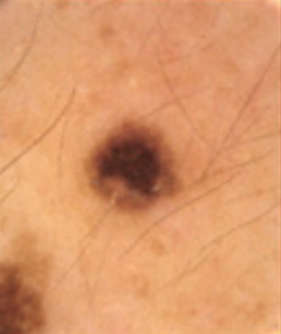
\includegraphics[height = 0.18\textheight, width= 0.16\textwidth]{Chapter2/Figures/quintana-calibrated_ex2.png}}
\caption[Color variations of dermoscopic images]{Variation in color depending on \Ac{awb}, \Ac{cwb} and \ac{jpeg} color calibration between images taken from two different dermoscopes. Images in the first row were taken with a Canon-A640 polarized dermoscope and the images in the second row were acquired with a Canon-G7 polarized dermoscope. Images are taken from~\cite{Quintana2011}.}
\label{fig:Quintana1}
\end{figure} 
 
\begin{figure}
\centering
\subfloat[\ac{cwb}]{
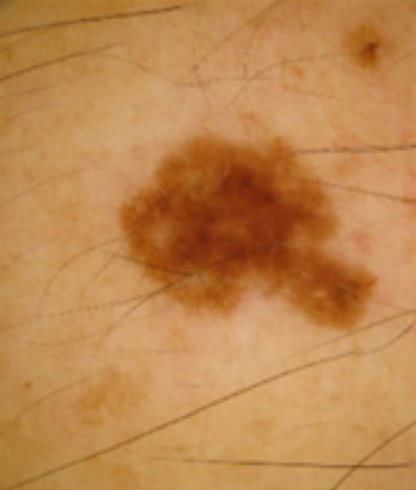
\includegraphics[height = 0.2\textheight, width= 0.19\textwidth]{Chapter2/Figures/quintana_cwb_ex3.png}}\
\subfloat[Calibrated-\ac{jpeg}]{
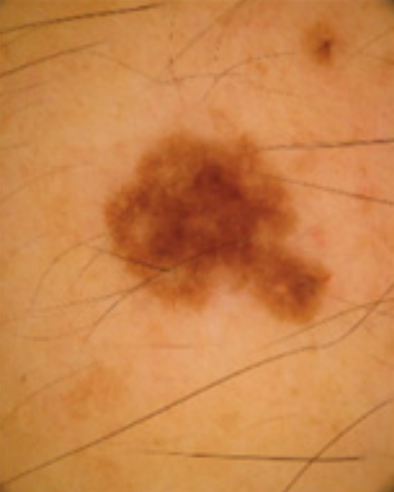
\includegraphics[height = 0.2\textheight, width= 0.19\textwidth]{Chapter2/Figures/quintana_JPEGCal_ex3.png}}\
\subfloat[Calibrated-RAW]{
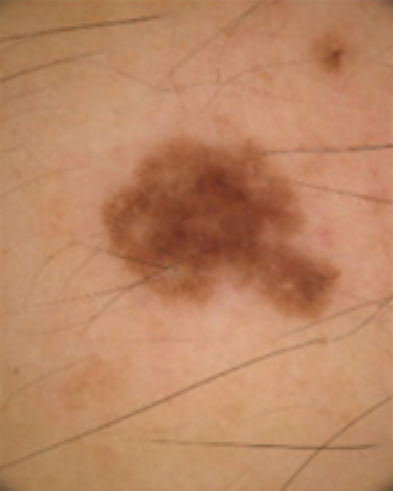
\includegraphics[height = 0.2\textheight, width= 0.19\textwidth]{Chapter2/Figures/quintana_RAWCal_ex3.png}}\\
\subfloat[\ac{cwb}]{
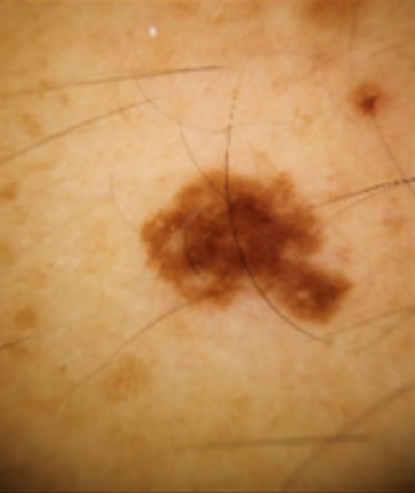
\includegraphics[height = 0.2\textheight, width= 0.19\textwidth]{Chapter2/Figures/quintana_cwb_ex4.png}}\
\subfloat[Calibrated-\ac{jpeg}]{
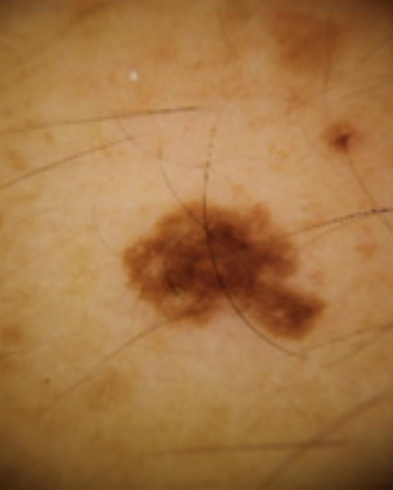
\includegraphics[height = 0.2\textheight, width= 0.19\textwidth]{Chapter2/Figures/quintana_JPEGCal_ex4.png}}
\subfloat[Calibrated-RAW]{
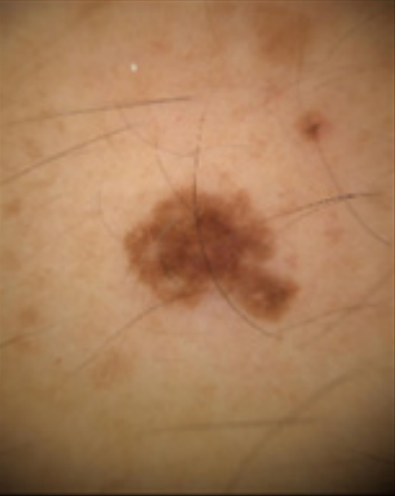
\includegraphics[height = 0.2\textheight, width= 0.19\textwidth]{Chapter2/Figures/quintana_RAWCal_ex4.png}}
\caption[Color variations between calibrated \ac{jpeg} and RAW images]{Variations in color between \Ac{cwb}, calibrated \ac{jpeg} and calibrated RAW images obtained with 2 different polarized dermoscopes. Images in the first row were acquired with Canon-G9 polarized dermoscope, while those in the second row were acquired with a Canon-5D polarized dermoscope. Images were taken from~\cite{Quintana2011}.}
\label{fig:Quintana2}
\end{figure}

\subsection{Artifacts removal} \label{subsec:artifactsremov}
Artifacts removal refers to noise removal in most image processing applications. 
However, in the field of skin imaging, it generally refers to elimination of hair, skin pores, ruler marks, air bubbles and specular reflections (see Fig.\ref{fig:artifacts}).
\begin{figure}
\centering
\subfloat[]{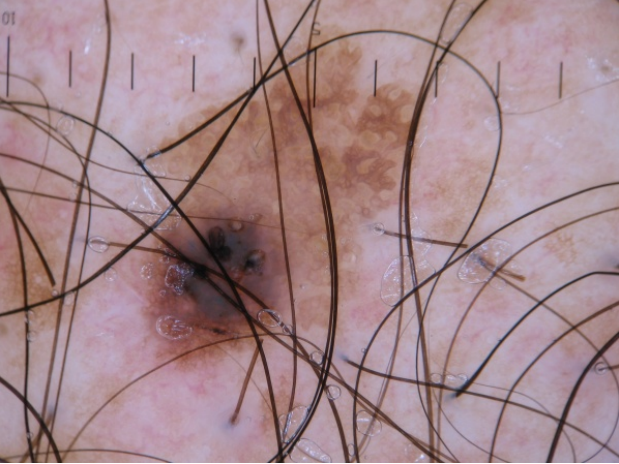
\includegraphics[height = 0.2\textheight, width= 0.3\textwidth]{Chapter2/Figures/artifacts-Hair-airbubble-Ruler.png}}\
\subfloat[]{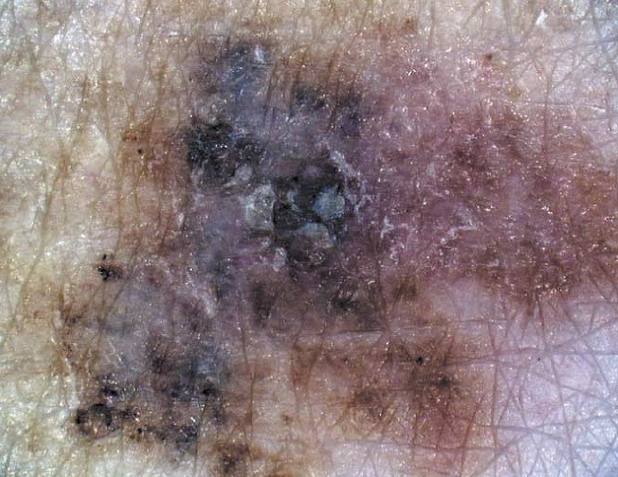
\includegraphics[height = 0.2\textheight, width= 0.3\textwidth]{Chapter2/Figures/artifacts-SpecularReflection.png}}
\caption[Artifacts in dermoscopic images]{Artifacts in dermoscopic images: (a) hair, air bubbles and ruler marks, (b) specular reflection. The images are taken from Zhou~et al.\,\cite{Zhou2008a} and Gutenev~et al.\,\cite{Gutenev2001}, respectively.}
\label{fig:artifacts}
\end{figure}
Among these operations, hair removal is the most common and necessary step.  
If a lesion is occluded by hairs, their removal is essential to achieve correct segmentation and texture analysis.
To avoid digital hair removal, the patients are usually asked to shave before image acquisition.

A hair removal algorithm commonly consists of two steps: hair detection and hair restoration (or ``inpainting'')~\cite{korotkov2012computerized}.
Inpainting fills the image space previously occupied by hairs with estimated intensity/color values. 
Considering that original colors and borders of a lesion play an essential role in lesion diagnosis, intensity estimation of missing pixels is crucial and the best inpainting method should be applied. 
\begin{figure}
\hspace*{\fill}
\subfloat[]{
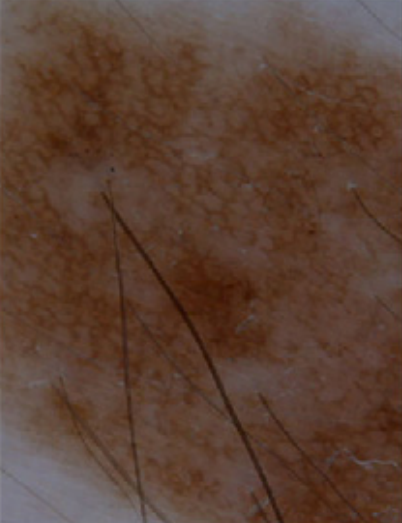
\includegraphics[height= 0.33\textheight, width= 0.3\textwidth]{Chapter2/Figures/Abas-comparison-original.png}}\hfill
\subfloat[]{
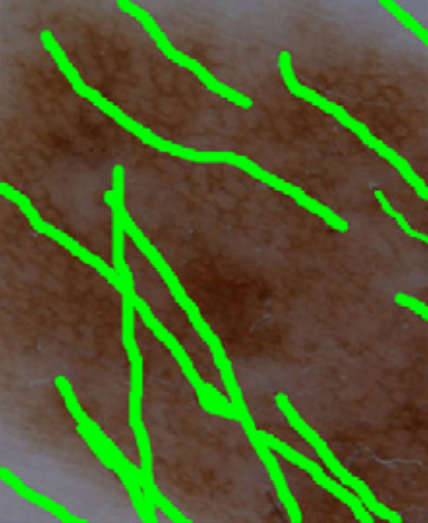
\includegraphics[height= 0.33\textheight, width= 0.3\textwidth]{Chapter2/Figures/Abas-comparison-mask.png}}\hfill
\subfloat[]{
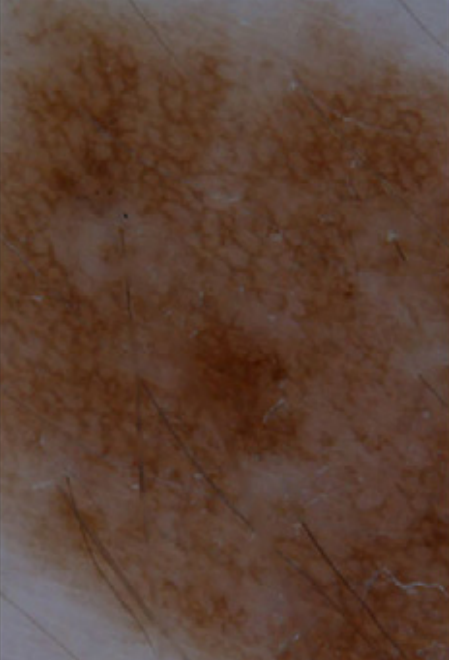
\includegraphics[height= 0.33\textheight, width= 0.3\textwidth]{Chapter2/Figures/Abas-comparison-dullruze.png}}
\hspace*{\fill}\\
\hspace*{\fill}
\subfloat[]{
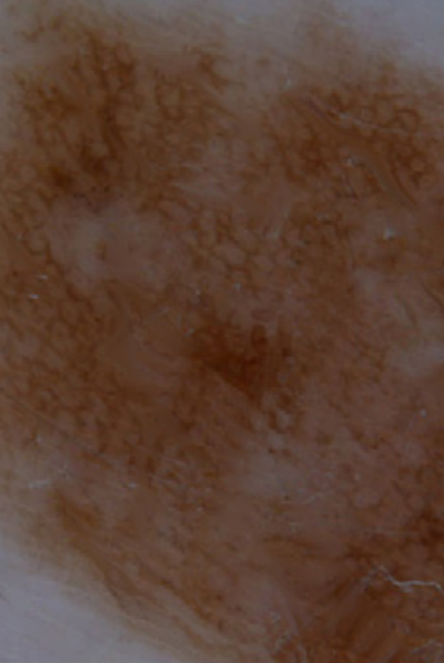
\includegraphics[height= 0.33\textheight, width= 0.3\textwidth]{Chapter2/Figures/Abas-comparison-d.png}}\hfill
\subfloat[]{
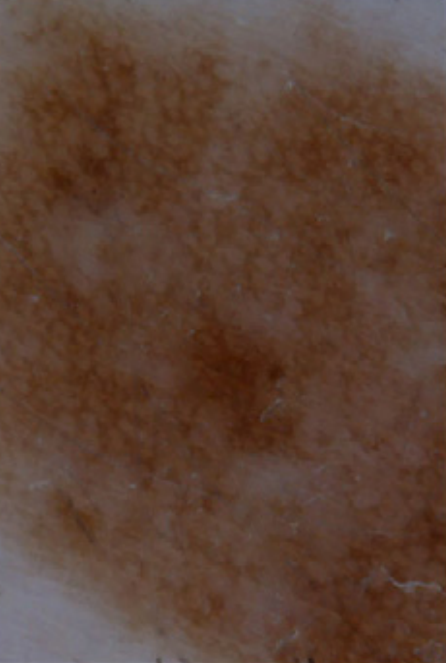
\includegraphics[height= 0.33\textheight, width= 0.3\textwidth]{Chapter2/Figures/Abas-comparison-e.png}}\hfill
\subfloat[]{
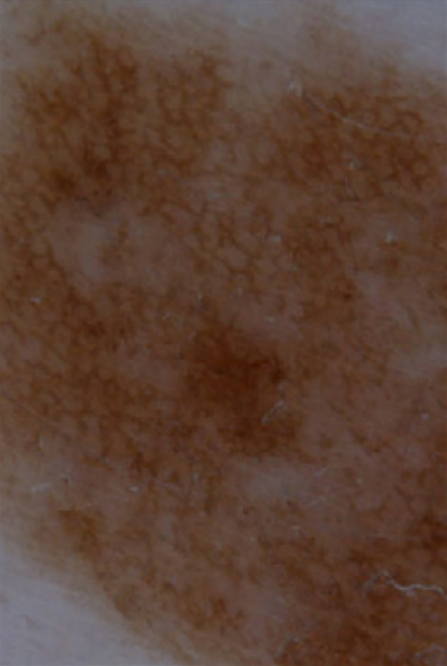
\includegraphics[height= 0.33\textheight, width= 0.3\textwidth]{Chapter2/Figures/Abas-comparison-fastmarching.png}}
\hspace*{\fill}
\caption[Comparison of inpainting methods]{Comparison of state of the art inpainting methods for hair removal algorithms. (a) Original image, (b) Highlighted hair mask, (c) DullRazor, (d) \ac{pde} non-linear inpainting, (e) exemplar-based inpainting, and (f) fast marching inpainting. The images are taken from \cite{Abbas2011a}.}
\label{fig:Abas-Comparison-repair}
\end{figure}
Lee~et al.\,\cite{Lee1997} proposed the first hair removal algorithm, DullRazor\textsuperscript{\textregistered}, for dermoscopic images. 
Kiani and Sharafat~\cite{Kiani2011} improved this algorithm to remove light-colored hairs as well as dark. 

Considering hair detection as a pixel classification problem, supervised learning was also applied in some studies~\cite{Debeir1999,Wighton2011}.
A recent survey on the topic was published by Abbas~et al.\,\cite{Abbas2011a}, where he reviewed the existing methods and proposed a broad classification based on the inpainting algorithms employed~\cite{korotkov2012computerized}: linear interpolation techniques~\cite{Lee1997,Fleming1998,Schmid-Saugeon2003,Nguyen2010}, inpainting by nonlinear \ac{pde}-based diffusion algorithms~\cite{Chung2000,Barcelos2009,Xie2009,Abbas2010a} and exemplar-based methods~\cite{Zhou2008a,Wighton2008,Abbas2010}. 
The authors~\cite{Abbas2011a,Abbas2012b} also proposed their own inpainting method based on fast marching inpainting. 
Figure~\ref{fig:Abas-Comparison-repair} shows an example demonstrating the results they achieved using different inpainting techniques.

\subsection{Image segmentation} \label{subsec:imgseg}
Image segmentation aims to decompose the image into meaningful parts with respect to a unique application. 
This technique uses image information such as grey level, texture, and color to divide the image into non-overlapping parts. 
Based on the information used, segmentation techniques are divided into four main groups: region-based, edge-based, clustering-based, and texture-based methods. 
Segmentation is also achievable via supervised learning. 

In automatic detection of melanoma, border delineation of the lesions is achieved by segmentation.
This is a challenging task due to variations in color, size, shape and texture of \ac{psls}, as well as occlusions and artifacts. 
In addition to the aforementioned challenges, segmentation algorithms face a problem of ground truth.  
%Moreover, due to difference of opinion among dermatologists and the fact that they do not require to delineate the lesion borders for their diagnosis~\cite{Day2001}, there is a ground truth problem.
It is very difficult to have a unique ground truth because dermatologists do not need to delineate lesion borders to make a diagnosis, and moreover, their individual delineations may vary significantly (see Fig.~\ref{fig:GTproblem}). 
So, normally the ground truth is generated as a fusion of different delineations done by experts. 
\begin{figure}
\centering
\subfloat[]{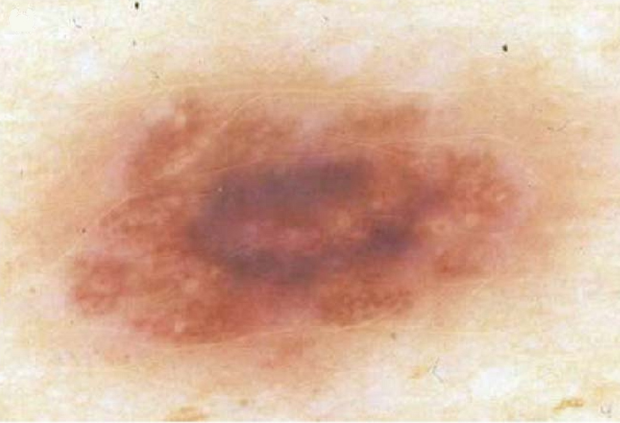
\includegraphics[height = 0.2\textheight, width= 0.3\textwidth]{Chapter2/Figures/Iyatomi-GT-original.png}}\	
\subfloat[]{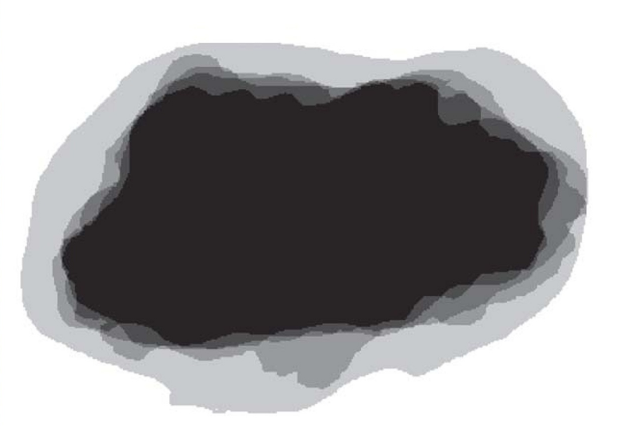
\includegraphics[height = 0.2\textheight, width= 0.3\textwidth]{Chapter2/Figures/Iyatomi-GT-5D.png}}
\caption[Lesion delineation variations]{Example of manual delineation of clark nevus by 5 dermatologists. (a) Dermoscopy image, (b) Delineation by 5 dermatologists. Images are taken from Iyatomi~et al.\,\cite{Iyatomi2006}.}
\label{fig:GTproblem}
\end{figure}
Despite these challenges, numerous methods were proposed by the research community to tackle this problem.
Good comparisons of segmentation methods for dermoscopy images were published by Silveira~et al.\,\cite{silveira2009comparison}, Celebi ~et al.\,\cite{Celebi2009a}, and Ferreira~et al.\,\cite{ferreira2013wide}.  %Korotkov~et al.\,\cite{korotkov2012computerized}
The proposed methods can be categorized based on different criteria, for instance, technical properties, level of automation or their complexity.
A review of all the proposed methods is beyond the scope of this research. 
However, an overview of available reviews and certain approaches is presented in the following.

Thresholding was one of the first approaches applied to lesion segmentation.
This technique was applied in a single color channel at first~\cite{Gutkowicz-Krusin1997,Fleming1998} and then evolved to more sophisticated approaches such as iterative thresholding~\cite{Rajab2004}, type-2 fuzzy logic based thresholding~\cite{Yuksel2009}, fusion of thresholds~\cite{Celebi2009c,Celebi2010, Celebi2013}, hybrid~\cite{Garnavi2011}, local entropy~\cite{Abbas2013a} and color histogram thresholding~\cite{Peruch2013}.

Among the many segmentation approaches developed, a variety of methods were employed such as clustering~\cite{Schmid1999b, Zhou2009, Mete2011, Liu2012}, active contours~\cite{Yuan2009, Zhou2011a,Erkol2005}, supervised learning~\cite{Debeir1999, Wighton2011, Wighton2011b, Zortea2011}, and dynamic programming~\cite{Abbas2012}, just to name a few~\cite{korotkov2012computerized}.

It is clear that without a common dataset, a comparison of the proposed methods cannot be made. 
In this regard, some studies surveyed a comparison of several methods on their own datasets~\cite{Hance1996,Silveira2009,Celebi2007,Celebi2008a,ferreira2013wide}.

Six segmentation methods (split-and-merge, center split, multiresolution, fuzzy c-mean, PCT/median cut and adaptive thresholding) were compared in~\cite{Hance1996}, where the two latter approaches outperformed the others~\cite{korotkov2012computerized}.
Silveira~et al.\,\cite{Silveira2009} also made a comparison of 6 different methods including the level set, adaptive thresholding, expectation-maximization level set, fuzzy-based split-and-merge, adaptive snakes and \ac{gvf} algorithms.
In their experiments, the best performance was achieved by the adaptive snakes algorithm.
%Melli~\textit{et al.}~\cite{Melli2006} compared the performance of color clustering techniques with the mean-shift algorithm obtaining the best score.

Celebi~et al.\,\cite{Celebi2007,Celebi2008a}, introduced and compared statistical regional merging (SRM) with optimized thresholding, orientation-sensitive c-means~\cite{Schmid1999b}, \ac{gvf}, a dermatologist-like tumor extraction (DTEA) algorithm~\cite{Iyatomi2006} and a JSEG algorithm~\cite{Celebi2007b}.
Their results indicated the superiority of SRM, followed by DTEA and JSEG~\cite{korotkov2012computerized}.
In another recent study, Ferreia~et al.\,\cite{ferreira2013wide} reported that the \ac{gvf} snakes outperformed the automatic thresholding, k-means, mean-shift, region growing and watershed algorithms. 
These comparisons still do not provide unified results, firstly due to the different datasets and ground truth employed, and secondly, to the different evaluation metrics~\cite{korotkov2012computerized}.


%- illumination correction 
%- hair removal 
%- segmentation 
